\documentclass[xetex,mathserif,serif]{beamer}
\usepackage{polyglossia}
\setdefaultlanguage[babelshorthands=true]{russian}
\usepackage{minted}
\usepackage{tabu}
\usepackage{moresize}

\useoutertheme{infolines}

\usepackage{fontspec}
\setmainfont{FreeSans}
\newfontfamily{\russianfonttt}{FreeSans}

\definecolor{links}{HTML}{2A1B81}
\hypersetup{colorlinks,linkcolor=,urlcolor=links}

\setbeamertemplate{blocks}[rounded][shadow=false]

\setbeamercolor*{block title alerted}{fg=red!50!black,bg=red!20}
\setbeamercolor*{block body alerted}{fg=black,bg=red!10}

\tabulinesep=1.2mm

\title{Введение, многопоточное программирование}
\author[Юрий Литвинов]{Юрий Литвинов\\\small{\textcolor{gray}{yurii.litvinov@gmail.com}}}
\date{06.09.2019г}

\newcommand{\attribution}[1] {
\vspace{-5mm}\begin{flushright}\begin{scriptsize}\textcolor{gray}{\textcopyright\, #1}\end{scriptsize}\end{flushright}
}

\begin{document}

	\frame{\titlepage}

	\section{Введение}

	\begin{frame}
		\frametitle{О чём этот курс}
		\begin{itemize}
			\item Кратко про почти всё, что обязательно знать любому прикладному программисту
			\begin{itemize}
				\item Многопоточное программирование
				\item Сетевое программирование
				\item Веб-программирование
				\item Продвинутое GUI-программирование
				\item Работа с базами данных
				\item Рефлексия
			\end{itemize}
			\item Язык программирования --- C\#
			\begin{itemize}
				\item Немного подробностей про внутреннее устройство .NET тоже будет в курсе
			\end{itemize}
		\end{itemize}
	\end{frame}

	\begin{frame}
		\frametitle{Отчётность}
		\begin{itemize}
			\item Домашка
			\item Две контрольные
			\item Доклады (-1 домашка) (если успеем)
			\item Учебная практика
		\end{itemize}
	\end{frame}

	\begin{frame}
		\frametitle{Учебная практика}
		\begin{itemize}
			\item Отдельный зачёт
			\item Программная реализация достаточно большой и полезной задачи
			\item Пишется весь семестр
			\item В конце --- защита с презентацией
			\item Может быть групповой
			\item Где брать темы
			\begin{itemize}
				\item Продолжать начатое в летней школе
				\item Студпроекты
				\item Придумать самим
				\item Взять что-нибудь у кого-нибудь поблизости
				\begin{itemize}
					\item Робототехника
					\item Формальные методы
					\item Machine Learning
				\end{itemize}
			\end{itemize}
			\item Гуглогруппа: \url{https://groups.google.com/forum/\#!forum/spbsu-se-bachelors-2018-2022}
		\end{itemize}
	\end{frame}

	\section{Многопоточность}

	\begin{frame}
		\frametitle{Многопоточное программирование}
		Зачем это нужно:
		\begin{itemize}
			\item Оптимально использовать ресурсы процессора
			\begin{itemize}
				\item Одноядерных процессоров практически не бывает
			\end{itemize}
			\item Использовать асинхронные операции ввода-вывода
			\item Не ``вешать'' GUI
			\item Показывать прогресс
		\end{itemize}
		\vspace{5mm}
		Потенциальные проблемы:
		\begin{itemize}
			\item Тысяча способов прострелить себе ногу
			\begin{itemize}
				\item Ошибки могут воспроизводиться раз в тысячу лет и их невозможно обнаружить статически
			\end{itemize}
			\item Не всегда многопоточная программа работает быстрее однопоточной
		\end{itemize}
	\end{frame}

	\begin{frame}
		\frametitle{Процессы и потоки}
		\begin{itemize}
			\item Процесс --- исполняющаяся программа
			\begin{itemize}
				\item Загруженный в память .exe-шник со всеми его .dll-ками или аналогичные понятия
				\item Имеет выделенные для него системные ресурсы:
				\begin{itemize}
					\item Память
					\item Открытые файлы
					\item Открытые сетевые соединения
					\item ...
				\end{itemize}
			\end{itemize}
			\item Поток --- единица параллельной работы
			\begin{itemize}
				\item Существует внутри процесса
				\item Имеет свой стек и состояние регистров процессора
				\item Все потоки внутри процесса разделяют общие ресурсы (например, память)
			\end{itemize}
		\end{itemize}
	\end{frame}

	\begin{frame}
		\frametitle{Параллельное программирование}
		\begin{itemize}
			\item Параллельная программа может быть:
			\begin{itemize}
				\item Многопроцессной
				\begin{itemize}
					\item Несколько процессов, возможно, несколько потоков в каждом
				\end{itemize}
				\item Многопоточной
			\end{itemize}
			\item Многопроцессные программы:
			\begin{itemize}
				\item Могут исполняться на разных компьютерах
				\item Пример --- веб-приложения
				\item Сложное и медленное взаимодействие между процессами
			\end{itemize}
			\item Многопоточные программы:
			\begin{itemize}
				\item Могут исполняться только на одном компьютере (нужна общая память)
				\item Быстрое общение между потоками через общую память
				\item Потоки могут портить состояние друг другу
			\end{itemize}
		\end{itemize}
	\end{frame}

	\section{Введение в устройство ОС}

	\begin{frame}
		\frametitle{Внезапно, операционные системы}
		Функции операционной системы:
		\begin{itemize}
			\item Предоставлять упрощённый доступ к оборудованию
			\begin{itemize}
				\item Файловая система
				\item Драйвера
			\end{itemize}
			\item Управлять ресурсами компьютера
			\begin{itemize}
				\item Виртуальная память
				\item Планировщик
			\end{itemize}
		\end{itemize}
	\end{frame}

	\begin{frame}
		\frametitle{Планировщик}
		\begin{itemize}
			\item Управляет распределением процессорного времени между процессами и потоками
			\item Каждому потоку выделяется квант времени, прерывание по таймеру
			\item Поток может отдать ядро процессора до истечения кванта
			\begin{itemize}
				\item Сам
				\item Блокирующая операция ввода-вывода
				\item Подгрузка страницы памяти из свопа
				\item Аппаратное прерывание
			\end{itemize}
			\item Хитрые алгоритмы планирования
			\begin{itemize}
				\item Обеспечение максимального быстродействия при справедливом планировании
				\item Учитываются приоритеты потоков
			\end{itemize}
		\end{itemize}
	\end{frame}

	\begin{frame}
		\frametitle{Планировщик в Windows}
		\begin{itemize}
			\item Раз в квант времени (или чаще) выбирает поток для исполнения
			\begin{itemize}
				\item Рассматриваются только потоки, не ждущие чего-либо
			\end{itemize}
			\item НЕ реальное время
			\begin{itemize}
				\item Нельзя делать предположения, когда потоку дадут поработать
			\end{itemize}
			\item Из рассматриваемых потоков выбираются только те, у кого наибольший приоритет
			\begin{itemize}
				\item Приоритеты потоков от 0 до 31, обычно 8
			\end{itemize}
			\item Есть ещё приоритеты процессов: Idle, Below, Normal, Normal, Above Normal, High и Realtime
			\item Относительные приоритеты потоков: Idle, Lowest, Below Normal, Normal, Above Normal, Highest и Time-Critical
			\begin{itemize}
				\item Истинный приоритет получается из относительного приоритета и приоритета процесса
			\end{itemize}
		\end{itemize}
	\end{frame}

	\begin{frame}
		\frametitle{Поток в Windows}
		\begin{itemize}
			\item Thread Kernel Object (\textasciitilde1240 байт)
			\item Thread environment block (TEB) (4 Кб)
			\item User-mode stack (1 Мб)
			\item Kernel-mode stack (24 Кб)
		\end{itemize}

		Ещё для каждой dll-ки, загруженной для процесса при старте или остановке потока, вызывается DllMain с параметрами DLL\_THREAD\_ATTACH и DLL\_THREAD\_DETACH

		\vspace{3mm}
		Квант времени --- \textasciitilde20-30 мс, после чего происходит \textit{переключение контекстов}
	\end{frame}

	\begin{frame}
		\frametitle{Как делать не надо}
		\begin{center}
			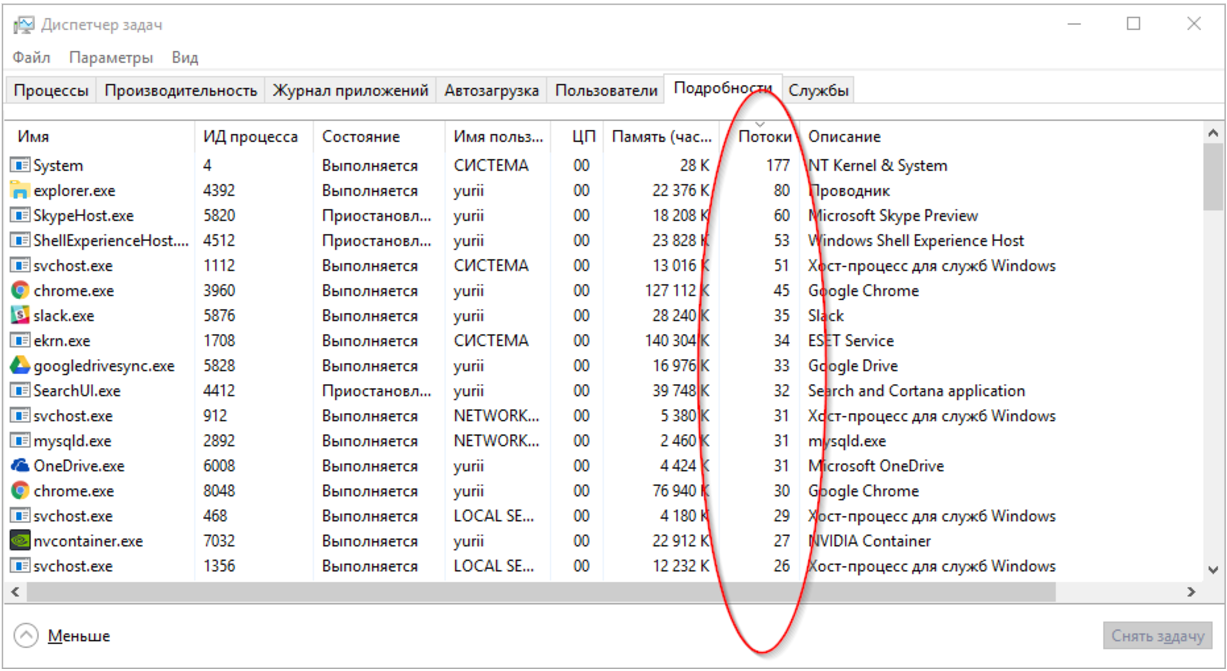
\includegraphics[width=0.9\textwidth]{threadsEverywhere.png}
		\end{center}
	\end{frame}

	\section{Потоки в .NET}

	\begin{frame}[fragile]
		\frametitle{System.Threading.Thread}
		\begin{footnotesize}
			\begin{minted}{csharp}
using System;
using System.Threading;

namespace MultiThreadingDemo {
    class Program {
        static void Main(string[] args) {
            var otherThread = new Thread(() => {
                while (true)
                    Console.WriteLine("Hello from other thread!");
            });
            otherThread.Start();

            while (true)
                Console.WriteLine("Hello from this thread!");
        }
    }
}
			\end{minted}
		\end{footnotesize}
	\end{frame}

	\begin{frame}[fragile]
		\frametitle{Параллельная обработка данных}
		\begin{ssmall}
			\begin{minted}{csharp}
static void Main(string[] args) {
    var array = new int[] { 1, 5, 2, 4, 7, 2, 4, 9, 3, 6, 5 };
    var threads = new Thread[3];
    var chunkSize = array.Length / threads.Length + 1;
    var results = new int[threads.Length];

    for (var i = 0; i < threads.Length; ++i) {
        var localI = i;
        threads[i] = new Thread(() => {
            for (var j = localI * chunkSize; j < (localI + 1) * chunkSize && j < array.Length; ++j)
                results[localI] += array[j];
        });
    }

    foreach (var thread in threads)
        thread.Start();
    foreach (var thread in threads)
        thread.Join();

    var result = 0;
    foreach (var subResult in results)
        result += subResult;

    Console.WriteLine($"Result = {result}");
}
			\end{minted}
		\end{ssmall}
	\end{frame}

	\section{Проблемы синхронизации}

	\begin{frame}[fragile]
		\frametitle{``Упрощённая'' версия}
		\begin{ssmall}
			\begin{minted}{csharp}
static void Main(string[] args) {
    var array = new int[] { 1, 5, 2, 4, 7, 2, 4, 9, 3, 6, 5 };
    var threads = new Thread[3];
    var chunkSize = array.Length / threads.Length + 1;
    var result = 0;

    for (var i = 0; i < threads.Length; ++i) {
        var localI = i;
        threads[i] = new Thread(() => {
            for (var j = localI * chunkSize; j < (localI + 1) * chunkSize && j < array.Length; ++j)
                result += array[j];
        });
    }

    foreach (var thread in threads)
        thread.Start();
    foreach (var thread in threads)
        thread.Join();

    Console.WriteLine($"Result = {result}");
}
			\end{minted}
		\end{ssmall}
	\end{frame}

	\begin{frame}[fragile]
		\frametitle{Немного увеличим размер задачи...}
		\begin{ssmall}
			\begin{minted}{csharp}
static void Main(string[] args) {
    var array = new int[1000];
    for (var i = 0; i < array.Length; ++i)
        array[i] = 1;

    var threads = new Thread[8];
    var chunkSize = array.Length / threads.Length + 1;
    var result = 0;

    for (var i = 0; i < threads.Length; ++i) {
        var localI = i;
        threads[i] = new Thread(() => {
            for (var j = localI * chunkSize; j < (localI + 1) * chunkSize && j < array.Length; ++j)
                result += array[j];
        });
    }

    foreach (var thread in threads)
        thread.Start();
    foreach (var thread in threads)
        thread.Join();

    Console.WriteLine($"Result = {result}");
}
			\end{minted}
		\end{ssmall}
	\end{frame}

	\begin{frame}[fragile]
		\frametitle{Почему так}
		\mintinline{csharp}|result += array[j];|

		\hspace{13mm}$\Downarrow$

		\begin{ssmall}
			\begin{minted}{text}
IL_0016: ldarg.0      // this
IL_0017: ldfld        class Program/'<>c__DisplayClass0_0' Program/'<>c__DisplayClass0_1'::'CS$<>8__locals1'
IL_001c: ldarg.0      // this
IL_001d: ldfld        class Program/'<>c__DisplayClass0_0' Program/'<>c__DisplayClass0_1'::'CS$<>8__locals1'
IL_0022: ldfld        int32 Program/'<>c__DisplayClass0_0'::result
IL_0027: ldarg.0      // this
IL_0028: ldfld        class Program/'<>c__DisplayClass0_0' Program/'<>c__DisplayClass0_1'::'CS$<>8__locals1'
IL_002d: ldfld        int32[] Program/'<>c__DisplayClass0_0'::'array'
IL_0032: ldloc.0      // j
IL_0033: ldelem.i4    
IL_0034: add          
IL_0035: stfld        int32 Program/'<>c__DisplayClass0_0'::result
			\end{minted}
		\end{ssmall}
		\vspace{5mm}
		Между \textbf{любыми} инструкциями поток может быть прерван
	\end{frame}

	\begin{frame}
		\frametitle{Race condition}
		\begin{center}
			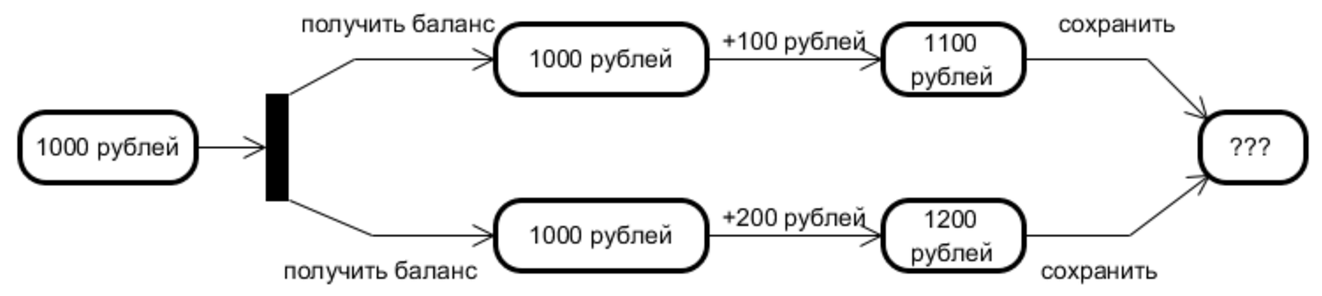
\includegraphics[width=0.9\textwidth]{raceCondition.png}
		\end{center}
	\end{frame}

	\begin{frame}
		\frametitle{Deadlock}
		\begin{center}
			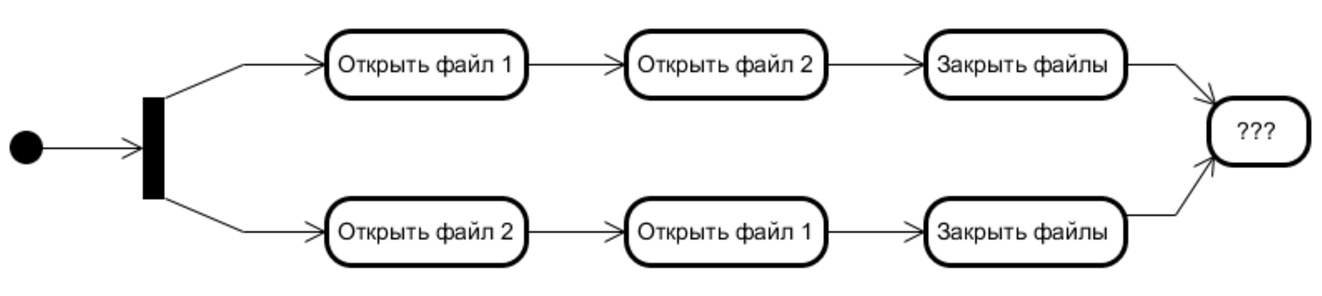
\includegraphics[width=0.9\textwidth]{deadlock.png}
		\end{center}
	\end{frame}

	\begin{frame}
		\frametitle{Какие ещё ловушки бывают}
		\begin{itemize}
			\item Процессор может переставлять местами инструкции
			\begin{itemize}
				\item Результат исполнения гарантируется таким же, как оригинальный, но промежуточные результаты другим 
					ядрам могут быть видны странные
			\end{itemize}
			\item У ядер процессора есть кеш (у каждого свой)
			\begin{itemize}
				\item На самом деле, обычно три уровня кеша: L1 и L2 для каждого ядра свой, L3 общий для всех ядер
				\item Кеши синхронизируются, но есть буферы чтения и записи, они нет
			\end{itemize}
		\end{itemize}
	\end{frame}

	\section{Синхронизация}

	\begin{frame}
		\frametitle{Примитивы синхронизации}
		\begin{itemize}
			\item Лучше необходимости синхронизации вообще избегать
			\item Бывают:
			\begin{itemize}
				\item User-mode --- атомарные операции, реализующиеся на процессоре и не требующие участия планировщика
				\item Kernel-mode --- примитивы, управляющие тем, как поток обрабатывается планировщиком
				\begin{itemize}
					\item Более тяжеловесные и медленные (до 1000 раз по сравнению с ``без синхронизации вообще'')
					\item Позволяют синхронизировать даже разные процессы
				\end{itemize}
			\end{itemize}
		\end{itemize}
	\end{frame}

	\begin{frame}
		\frametitle{Атомарные операции}
		\begin{itemize}
			\item Чтения и записи следующих типов всегда атомарны: Boolean, Char, (S)Byte, (U)Int16, (U)Int32, (U)IntPtr, Single, ссылочные типы
			\item Для других типов (например, Int64) операции чтения и записи могут быть прерваны посередине!
			\item \mintinline{csharp}|Volatile|
			\begin{itemize}
				\item \mintinline{csharp}|Volatile.Write|
				\item \mintinline{csharp}|Volatile.Read|
				\item Связано с понятием Memory Fence, требует синхронизации ядер
				\item Есть ключевое слово \mintinline{csharp}|volatile|: \mintinline{csharp}|private volatile int flag = 0;|
				\item \mintinline{csharp}|Volatile.Write| должен быть последней операцией записи, \mintinline{csharp}|Volatile.Read| --- первой операцией чтения
			\end{itemize}
			\item Про это подробнее ближе к концу семестра, но volatile потребуется в домашке
		\end{itemize}
	\end{frame}

	\begin{frame}[fragile]
		\frametitle{Пример}
		\begin{minted}{csharp}
private int flag = 0;
private int value = 0;

public void Thread1() {
    value = 5;
    Volatile.Write(ref flag, 1);
}

public void Thread2() {
    if (Volatile.Read(ref flag) == 1)
        Console.WriteLine(value);
}
		\end{minted}
	\end{frame}

	\section{Синхронизация уровня ОС}

	\begin{frame}
		\frametitle{Критические области}
		\begin{center}
			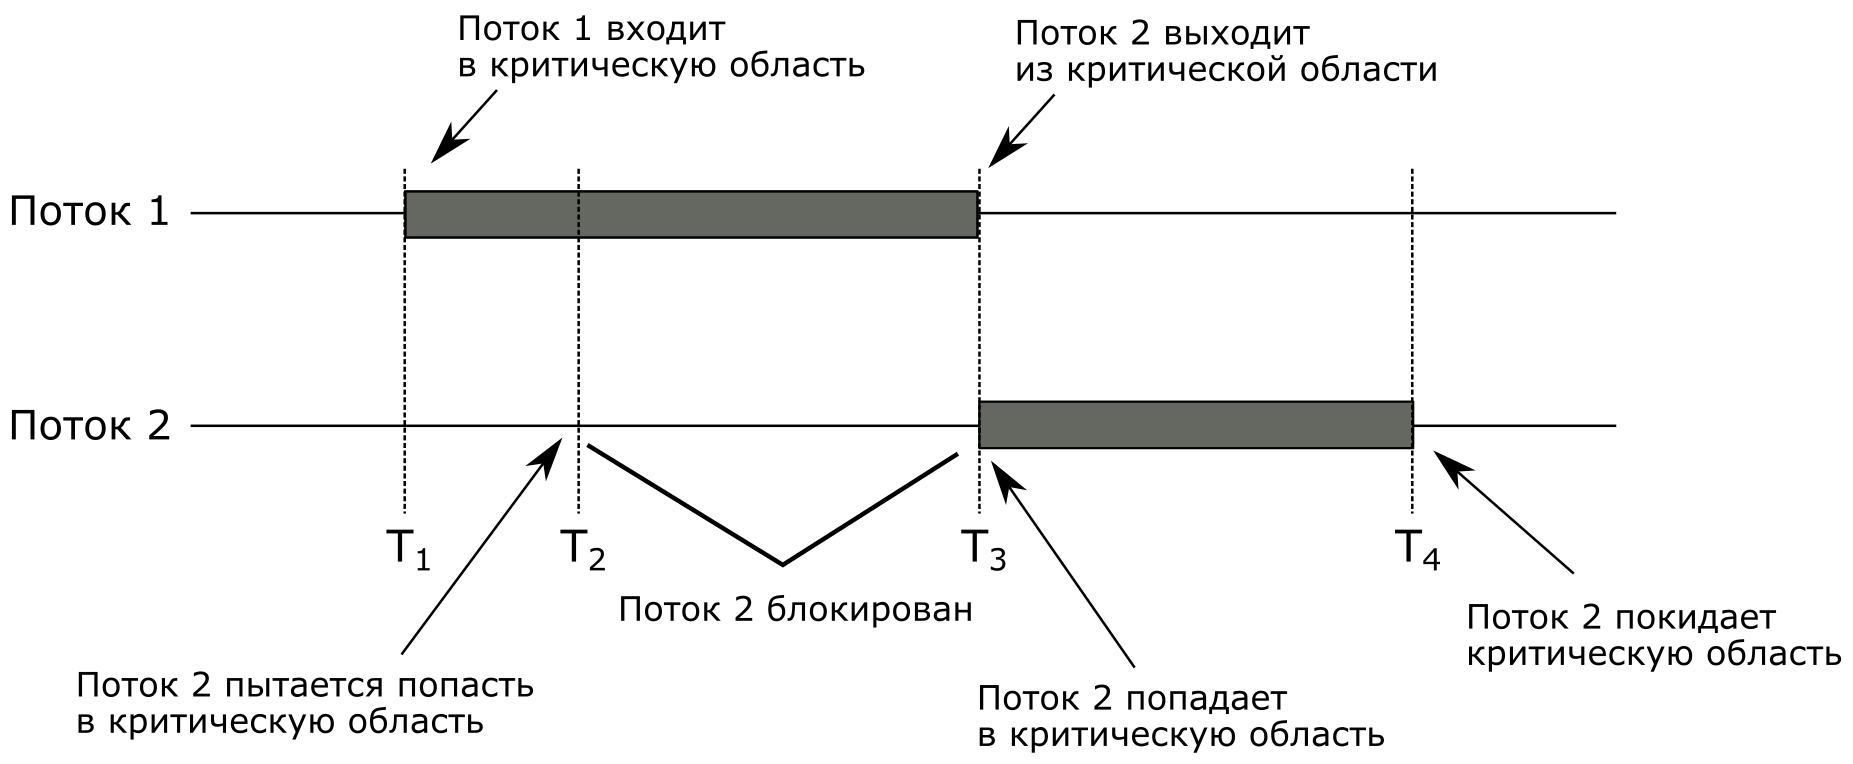
\includegraphics[width=0.9\textwidth]{criticalSections.png}
		\end{center}
	\end{frame}

	\begin{frame}[fragile]
		\frametitle{Активное ожидание}
		\begin{scriptsize}
			\begin{minted}{csharp}
private int turn = 0;

void Task1()
{
    while (true)
    {
        while (turn != 0) ;
        CriticalSection();
        turn = 1;
        NonCriticalSection();
    }
}

void Task2()
{
    while (true)
    {
        while (turn != 1) ;
        CriticalSection();
        turn = 0;
        NonCriticalSection();
    }
}
			\end{minted}
		\end{scriptsize}
	\end{frame}

	\begin{frame}
		\frametitle{Активное ожидание, обсуждение}
		\begin{itemize}
			\item Не требует поддержки ОС
			\begin{itemize}
				\item Поэтому переключение может быть очень быстрым
			\end{itemize}
			\item Ждущий поток полностью занимает ядро
			\begin{itemize}
				\item Греет процессор и очень быстро сажает аккумулятор
			\end{itemize}
			\item Потоки работают строго по очереди
			\begin{itemize}
				\item Это можно побороть, есть алгоритм Петерсона
			\end{itemize}
		\end{itemize}
	\end{frame}

	\begin{frame}[fragile]
		\frametitle{Проблема производителя и потребителя}
		\framesubtitle{Producer-consumer problem}
		\begin{footnotesize}
			\begin{minted}{csharp}
private Queue<int> buffer = new Queue<int>();
			\end{minted}
			\begin{columns}
				\begin{column}{0.5\textwidth}
					\begin{minted}{csharp}
private void Producer() {
    while (true) {
        var item = ProduceItem();
        if (buffer.Count == 100)
            Sleep();
        buffer.Enqueue(item);
        if (buffer.Count == 1)
            WakeUp(Consumer);
    }
}
					\end{minted}
				\end{column}
				\begin{column}{0.5\textwidth}
					\begin{minted}{csharp}
private void Consumer() {
    while (true) {
        if (buffer.Count == 0)
            Sleep();
        var item = buffer.Dequeue();
        if (buffer.Count == 100 - 1)
            WakeUp(Producer);
        ConsumeItem(item);
    }
}
					\end{minted}
				\end{column}
			\end{columns}
		\end{footnotesize}
	\end{frame}

	\begin{frame}[fragile]
		\frametitle{Семафоры}
		\framesubtitle{Дейкстры (того самого), 1965 год}
		\begin{itemize}
			\item Целочисленный счётчик, который можно поднять и опустить (\textbf{up()} и \textbf{down()})
			\item \textbf{down()} уменьшает счётчик на 1, если он больше нуля или блокирует вызывающего, если он 0
			\item \textbf{up()} увеличивает счётчик на один и, если он был нулём, будит одного из ожидающих потоков (случайного!)
			\item \textbf{down()} обычно делается при входе в критическую секцию, \textbf{up()} --- при выходе
			\item Позволяет быть в критической секции не более чем заданному количеству потоков
			\begin{itemize}
				\item Например, Google Drive не позволяет качать более чем с 10 подключениями одновременно, семафор решает проблему
			\end{itemize}
		\end{itemize}
	\end{frame}

	\begin{frame}[fragile]
		\frametitle{Производитель-потребитель на семафорах}
		\begin{footnotesize}
			\begin{minted}{csharp}
private Queue<int> buffer = new Queue<int>();
private Semaphore mutex = new Semaphore(0, 1);
private Semaphore empty = new Semaphore(100, 100);
private Semaphore full = new Semaphore(0, 100);
			\end{minted}
			\begin{columns}
				\begin{column}{0.5\textwidth}
					\begin{minted}{csharp}
private void Producer()
{
    while (true)
    {
        var item = ProduceItem();
        empty.WaitOne();
        mutex.WaitOne();
        buffer.Enqueue(item);
        mutex.Release();
        full.Release();
    }
}
					\end{minted}
				\end{column}
				\begin{column}{0.5\textwidth}
					\begin{minted}{csharp}
private void Consumer()
{
    while (true)
    {
        full.WaitOne();
        mutex.WaitOne();
        var item = buffer.Dequeue();
        mutex.Release();
        empty.Release();
        ConsumeItem(item);
    }
}
					\end{minted}
				\end{column}
			\end{columns}
		\end{footnotesize}
	\end{frame}

	\begin{frame}
		\frametitle{Мьютекс}
		\begin{itemize}
			\item Мьютекс --- бинарный семафор
			\begin{itemize}
				\item Пускает ровно один поток в критическую секцию
			\end{itemize}
			\item Существенно проще в реализации и использовании, чем семафор
			\item Тоже требует поддержки операционной системы
			\begin{itemize}
				\item Может использоваться для синхронизации даже процессов
			\end{itemize}
		\end{itemize}
	\end{frame}

	\begin{frame}[fragile]
		\frametitle{Производитель-потребитель на семафорах и мьютексе}
		\begin{footnotesize}
			\begin{minted}{csharp}
private Queue<int> buffer = new Queue<int>();
private Mutex mutex = new Mutex();
private Semaphore empty = new Semaphore(100, 100);
private Semaphore full = new Semaphore(0, 100);
			\end{minted}
			\begin{columns}
				\begin{column}{0.5\textwidth}
					\begin{minted}{csharp}
private void Producer()
{
    while (true)
    {
        var item = ProduceItem();
        empty.WaitOne();
        mutex.WaitOne();
        buffer.Enqueue(item);
        mutex.ReleaseMutex();
        full.Release();
    }
}
					\end{minted}
				\end{column}
				\begin{column}{0.5\textwidth}
					\begin{minted}{csharp}
private void Consumer()
{
    while (true)
    {
        full.WaitOne();
        mutex.WaitOne();
        var item = buffer.Dequeue();
        mutex.ReleaseMutex();
        empty.Release();
        ConsumeItem(item);
    }
}
					\end{minted}
				\end{column}
			\end{columns}
		\end{footnotesize}
	\end{frame}

	\begin{frame}
		\frametitle{Монитор}
		\framesubtitle{Хоара, 1974 год}
		\begin{itemize}
			\item Пользоваться семафорами очень сложно --- например, поменять empty.WaitOne(); и mutex.WaitOne(); в Producer() --- хороший способ устроить дедлок
			\begin{itemize}
				\item Представим, что буфер полон. Producer() захватывает мьютекс и встаёт на семафоре empty, потому что он 0, управление передаётся Consumer(). Он тут же встаёт на mutex.WaitOne(), потому что он захвачен Producer()-ом. Теперь оба потока ждут друг друга.
			\end{itemize}
			\item Поэтому придумали мониторы
			\item Монитор --- набор методов (или функций), внутри которых может находиться ровно один поток
			\item Реализуется через мьютексы, требует поддержки в языке программирования
		\end{itemize}
	\end{frame}

	\begin{frame}[fragile]
		\frametitle{Производитель-потребитель на мониторе}
		\begin{scriptsize}
			\begin{columns}
				\begin{column}{0.5\textwidth}
					\begin{minted}{csharp}
private class SynchronizedQueue {
    private Queue<int> buffer = 
        new Queue<int>();

    public void Enqueue(int item) {
        lock (buffer) {
            while (buffer.Count == 100)
                Monitor.Wait(buffer);
            buffer.Enqueue(item);
            Monitor.Pulse(buffer);
        }
    }

    public int Dequeue() {
        lock (buffer) {
            while (buffer.Count == 0)
                Monitor.Wait(buffer);
            var result = buffer.Dequeue();
            Monitor.Pulse(buffer);
            return result;
        }
    }
}
					\end{minted}
				\end{column}
				\begin{column}{0.5\textwidth}
					\begin{minted}{csharp}
private SynchronizedQueue buffer = 
    new SynchronizedQueue();

private void Producer() {
    while (true) {
        var item = ProduceItem();
        buffer.Enqueue(item);
    }
}

private void Consumer() {
    while (true) {
        var item = buffer.Dequeue();
        ConsumeItem(item);
    }
}
					\end{minted}
				\end{column}
			\end{columns}
		\end{scriptsize}
	\end{frame}

	\begin{frame}[fragile]
		\frametitle{lock в .NET}
		\begin{itemize}
			\item У каждого объекта (сылочного типа) есть скрытое поле, указывающее на структуру синхронизации
			\item lock использует именно её
			\begin{itemize}
				\item То есть lock в одной критической секции, но на разные объекты --- это разные мониторы
				\item Но lock в разных секциях на один объект --- один монитор
				\item lock умеет обрабатывать исключения и отпускать замок
				\begin{itemize}
					\item Предыдущие примеры с семафорами и мьютексами были неправильными --- не учитывались исключения
				\end{itemize}
			\end{itemize}
			\item Хорошая практика --- создавать объект специально для синхронизации, \mintinline{csharp}|lock(this)| писать нельзя!
		\end{itemize}
		\begin{footnotesize}
			\begin{minted}{csharp}
private Object lockObject = new Object();

private void SomeMethod() {
    lock (lockObject) {
        ...
    }
}
			\end{minted}
		\end{footnotesize}
	\end{frame}

	\begin{frame}
		\frametitle{WaitHandle}
		\begin{itemize}
			\item \mintinline{csharp}|WaitHandle| --- всё, что можно ожидать
			\begin{itemize}
				\item \mintinline{csharp}|EventWaitHandle|
				\begin{itemize}
					\item \mintinline{csharp}|AutoResetEvent| --- по сути, булевый флаг, поддерживаемый ОС
					\item \mintinline{csharp}|ManualResetEvent| --- тоже булевый флаг, но сбрасывается вручную
				\end{itemize}
			\end{itemize}
			\item Остальные примитивы синхронизации --- наследники WaitHandle
		\end{itemize}
	\end{frame}

	\begin{frame}[fragile]
		\frametitle{Пример (самодельный замок на Event-ах)}
		\begin{small}
			\begin{minted}{csharp}
internal class SimpleWaitLock : IDisposable {
    private readonly AutoResetEvent available;
    public SimpleWaitLock() {
        available = new AutoResetEvent(true); 
    }

    public void Enter() {
        available.WaitOne();
    }

    public void Leave() {
        available.Set();
    }

    public void Dispose() { available.Dispose(); }
}
			\end{minted}
		\end{small}
	\end{frame}

	\begin{frame}
		\frametitle{Литература}
		\begin{columns}
			\begin{column}{0.6\textwidth}
				Эндрю Таненбаум, Х. Бос, Современные операционные системы, Питер, 2017. 1120 С.
			\end{column}
			\begin{column}{0.3\textwidth}
				\begin{center}
					
\includegraphics[width=0.6\textwidth]{tannenbaumCover.png}
				\end{center}
			\end{column}
		\end{columns}
		\begin{columns}
			\begin{column}{0.6\textwidth}
				Jeffrey Richter, CLR via C\# (4th Edition), Microsoft Press, 2012. 894pp.
			\end{column}
			\begin{column}{0.3\textwidth}
				\begin{center}
					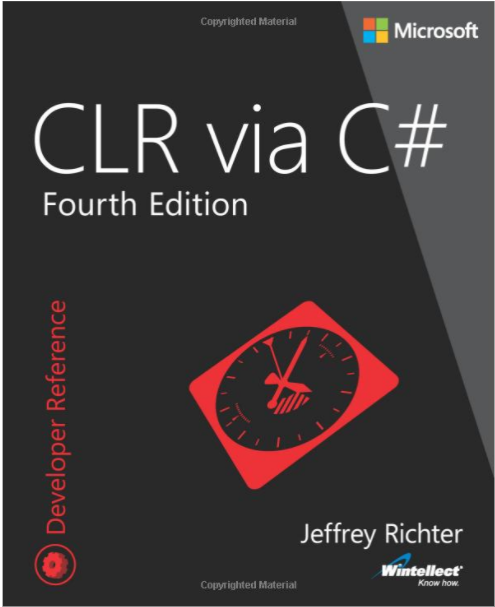
\includegraphics[width=0.6\textwidth]{clrViaCSharpCover.png}
				\end{center}
			\end{column}
		\end{columns}
	\end{frame}


\end{document}
